\documentclass[10pt]{beamer}
\usepackage[utf8]{inputenc}
\usepackage{graphicx}
\usepackage{listings}
\usepackage{xcolor}
\usepackage{tikz}
\usepackage{amsmath}
\usepackage{amsfonts}
\usepackage{amssymb}
\usepackage{url}
\usepackage{hyperref}

% Theme configuration
\usetheme{Madrid}
\usecolortheme{default}

% Color definitions
\definecolor{codebackground}{rgb}{0.95,0.95,0.95}
\definecolor{commentcolor}{rgb}{0.0,0.5,0.0}
\definecolor{keywordcolor}{rgb}{0.0,0.0,1.0}
\definecolor{stringcolor}{rgb}{0.6,0.0,0.0}

% Code listing style
\lstset{
    backgroundcolor=\color{codebackground},
    basicstyle=\ttfamily\footnotesize,
    keywordstyle=\color{keywordcolor}\bfseries,
    stringstyle=\color{stringcolor},
    commentstyle=\color{commentcolor}\itshape,
    numbers=left,
    numberstyle=\tiny,
    numbersep=5pt,
    breaklines=true,
    showstringspaces=false,
    tabsize=2,
    frame=single,
    language=C++
}

% Title page information
\title[CSOPESY OS Emulator]{CSOPESY Operating System Emulator}
\subtitle{Advanced OS Concepts Implementation in C++20}
\author[PEGP Team]{Paul Ivan Enclonar, Joel Ethan Batac, Joshua Gilo, Peter Parker}
\institute[CSOPESY]{Computer Systems Organization and Programming}
\date{\today}

\begin{document}

% Title slide
\begin{frame}
    \titlepage
\end{frame}

% Table of contents
\begin{frame}{Outline}
    \tableofcontents
\end{frame}

% ======================================================
% SECTION 1: SYSTEM OVERVIEW
% ======================================================
\section{System Overview}

\begin{frame}{System Architecture Overview}
    \begin{itemize}
        \item \textbf{Language:} C++20 with advanced features
        \item \textbf{Build System:} CMake with modern C++ standards
        \item \textbf{Architecture:} Multi-threaded OS simulation
        \item \textbf{Core Features:}
        \begin{itemize}
            \item Virtual memory with demand paging
            \item Multi-core CPU scheduling
            \item Process management with PCB
            \item Memory management with LRU replacement
            \item Command-line interface system
        \end{itemize}
    \end{itemize}
    
    \vspace{0.5cm}
    \begin{center}
        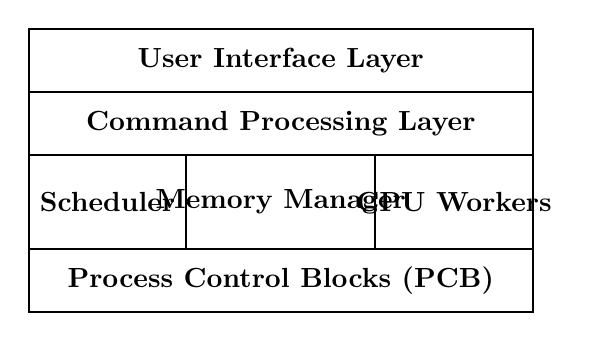
\begin{tikzpicture}[scale=0.8]
            \draw[thick] (0,0) rectangle (8,1);
            \node at (4,0.5) {\textbf{User Interface Layer}};
            
            \draw[thick] (0,-1) rectangle (8,0);
            \node at (4,-0.5) {\textbf{Command Processing Layer}};
            
            \draw[thick] (0,-2.5) rectangle (2.5,-1);
            \node at (1.25,-1.75) {\textbf{Scheduler}};
            
            \draw[thick] (2.5,-2.5) rectangle (5.5,-1);
            \node at (4,-1.75) {\textbf{Memory Manager}};
            
            \draw[thick] (5.5,-2.5) rectangle (8,-1);
            \node at (6.75,-1.75) {\textbf{CPU Workers}};
            
            \draw[thick] (0,-3.5) rectangle (8,-2.5);
            \node at (4,-3) {\textbf{Process Control Blocks (PCB)}};
        \end{tikzpicture}
    \end{center}
\end{frame}

\begin{frame}{System Data Flow}
    \begin{center}
        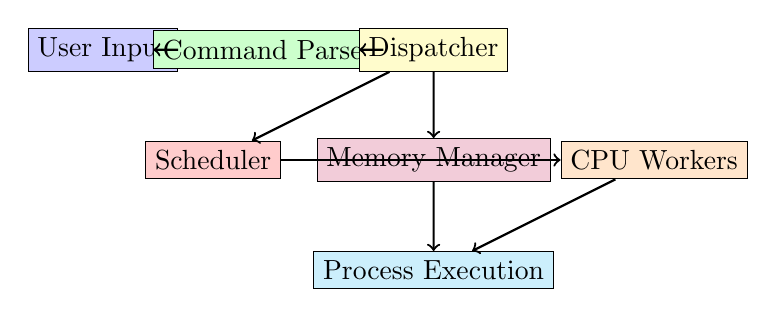
\begin{tikzpicture}[scale=0.7]
            % User Input
            \node[draw, rectangle, fill=blue!20] (input) at (0,4) {User Input};
            
            % Command Parser
            \node[draw, rectangle, fill=green!20] (parser) at (3,4) {Command Parser};
            
            % Dispatcher
            \node[draw, rectangle, fill=yellow!20] (dispatcher) at (6,4) {Dispatcher};
            
            % Scheduler
            \node[draw, rectangle, fill=red!20] (scheduler) at (2,2) {Scheduler};
            
            % Memory Manager
            \node[draw, rectangle, fill=purple!20] (memory) at (6,2) {Memory Manager};
            
            % CPU Workers
            \node[draw, rectangle, fill=orange!20] (cpu) at (10,2) {CPU Workers};
            
            % Process Execution
            \node[draw, rectangle, fill=cyan!20] (execution) at (6,0) {Process Execution};
            
            % Arrows
            \draw[->, thick] (input) -- (parser);
            \draw[->, thick] (parser) -- (dispatcher);
            \draw[->, thick] (dispatcher) -- (scheduler);
            \draw[->, thick] (dispatcher) -- (memory);
            \draw[->, thick] (scheduler) -- (cpu);
            \draw[->, thick] (memory) -- (execution);
            \draw[->, thick] (cpu) -- (execution);
        \end{tikzpicture}
    \end{center}
\end{frame}

% ======================================================
% SECTION 2: CORE COMPONENTS
% ======================================================
\section{Core Components}

\begin{frame}[fragile]{Process Control Block (PCB)}
    \textbf{Core Data Structure for Process Management}
    \begin{lstlisting}[language=C++]
class PCB {
    std::atomic<uint32_t> processID;           // Unique identifier
    std::string processName;                   // Process name
    std::atomic<size_t> currentInstruction;   // Instruction pointer
    size_t totalInstructions;                 // Total instruction count
    std::optional<int> assignedCore;          // CPU core assignment
    std::vector<Expr> instructions;           // Parsed instruction sequence
    std::unordered_map<std::string, uint16_t> symbol_table; // Variables
    std::vector<std::string> output_log;      // Execution history
    std::unique_ptr<InstructionEvaluator> evaluator; // Processor
    uint16_t sleepCyclesRemaining;           // Sleep state
    bool terminated_;                         // Termination status
    size_t memory_size_;                     // Virtual memory size
};
    \end{lstlisting}
\end{frame}

\begin{frame}[fragile]{PCB Key Methods}
    \textbf{Critical Process Management Operations}
    \begin{lstlisting}[language=C++]
// Execute one instruction cycle with page fault handling
bool step(MemoryManager& mm);

// Core execution engine with exception handling
bool executeCurrentInstruction(MemoryManager& mm);

// Process completion detection
bool isComplete() const;

// Process termination with reason logging
void terminate(const std::string& reason);

// Get formatted status string for reports
std::string status() const;
    \end{lstlisting}
    
    \vspace{0.3cm}
    \textbf{Memory Integration Features:}
    \begin{itemize}
        \item Symbol table manages variable-to-address mappings
        \item 64-byte stack at top of virtual memory space
        \item Virtual memory operations through MemoryManager
        \item Page fault exception handling and recovery
    \end{itemize}
\end{frame}

\begin{frame}[fragile]{Scheduler Architecture}
    \textbf{Multi-Core Process Scheduling System}
    \begin{lstlisting}[language=C++]
class Scheduler {
    std::vector<std::unique_ptr<CpuWorker>> cpu_workers_;     // Multi-core
    ThreadSafeQueue<std::shared_ptr<PCB>> ready_queue_;       // Process queue
    std::unique_ptr<MemoryManager> memory_manager_;           // Memory system
    std::atomic<bool> running_;                               // System state
    std::atomic<bool> batch_generating_;                      // Process gen
    std::atomic<size_t> ticks_, idle_ticks_, active_ticks_;  // Statistics
    
    // Thread management
    std::thread dispatch_thread_;        // Process dispatching
    std::thread global_clock_thread_;    // System timing
    std::unique_ptr<std::thread> batch_generator_thread_; // Process gen
};
    \end{lstlisting}
\end{frame}

\begin{frame}[fragile]{Scheduler Key Operations}
    \textbf{Core Scheduling Methods}
    \begin{lstlisting}[language=C++]
// Core scheduling loop with idle worker detection
void dispatch();

// System tick management with CPU utilization tracking
void global_clock();

// Lifecycle management with thread coordination
void start() / stop();

// Process submission with admission control
void submit_process(std::shared_ptr<PCB> pcb);

// Virtual memory statistics generation
std::string generate_vmstat_report();
    \end{lstlisting}
    
    \vspace{0.3cm}
    \textbf{Scheduling Algorithms:}
    \begin{itemize}
        \item \textbf{FCFS:} Quantum = -1 (unlimited execution time)
        \item \textbf{Round Robin:} Configurable quantum with preemptive scheduling
        \item \textbf{Load Balancing:} Automatic distribution across CPU cores
    \end{itemize}
\end{frame}

\begin{frame}[fragile]{CPU Worker Implementation}
    \textbf{Thread-Based CPU Core Simulation}
    \begin{lstlisting}[language=C++]
class CpuWorker {
    const int core_id_;                    // Core identifier
    Scheduler& scheduler_;                 // Parent scheduler reference
    std::thread thread_;                   // Worker execution thread
    std::atomic<bool> is_idle_;           // Idle state tracking
    std::shared_ptr<PCB> current_task_;   // Currently assigned process
    int time_quantum_;                    // Time slice allocation
};
    \end{lstlisting}
    
    \vspace{0.3cm}
    \textbf{Execution Flow:}
    \begin{enumerate}
        \item \textbf{Wait State:} Condition variable wait for task assignment
        \item \textbf{Task Execution:} Process execution with quantum management
        \item \textbf{Progress Detection:} Deadlock prevention with timeout mechanisms
        \item \textbf{State Management:} Idle/busy state transitions
        \item \textbf{Page Fault Handling:} Fault detection and recovery
    \end{enumerate}
\end{frame}

% ======================================================
% SECTION 3: MEMORY MANAGEMENT
% ======================================================
\section{Memory Management}

\begin{frame}[fragile]{Virtual Memory Architecture}
    \textbf{Advanced Memory Management System}
    \begin{lstlisting}[language=C++]
struct PageTableEntry {
    bool is_valid = false;      // Page presence in memory
    bool is_dirty = false;      // Modified page flag
    bool is_referenced = false; // Access tracking for LRU
    uint32_t frame_id = 0;      // Physical frame mapping
};

struct Frame {
    uint32_t id;               // Frame identifier
    uint32_t pcb_id = 0;       // Owning process
    uint32_t page_id = 0;      // Virtual page number
    bool is_free = true;       // Allocation status
};
    \end{lstlisting}
    
    \vspace{0.3cm}
    \textbf{Key Features:}
    \begin{itemize}
        \item Demand paging with lazy loading
        \item LRU page replacement algorithm
        \item File-based backing store system
        \item Process isolation and memory protection
    \end{itemize}
\end{frame}

\begin{frame}[fragile]{Memory Management Operations}
    \textbf{Critical Memory System Methods}
    \begin{lstlisting}[language=C++]
// Virtual to physical address translation
uint32_t translate_address(uint32_t pcb_id, uint32_t virtual_address, 
                          bool is_write);

// Page fault handling with demand loading
void handle_page_fault(uint32_t pcb_id, uint32_t page_id);

// LRU page replacement algorithm
uint32_t find_victim_frame();

// Backing store operations
void save_page_to_backing_store(uint32_t frame_id, uint32_t pcb_id, 
                               uint32_t page_id);
void load_page_from_backing_store(uint32_t frame_id, uint32_t pcb_id, 
                                 uint32_t page_id);
    \end{lstlisting}
\end{frame}

\begin{frame}{Memory Management Architecture}
    \begin{center}
        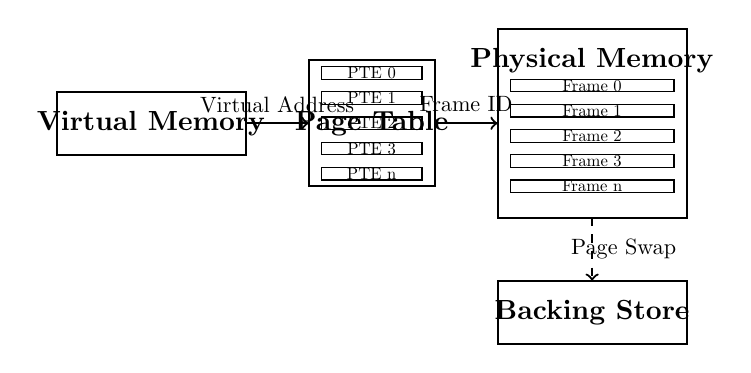
\begin{tikzpicture}[scale=0.8]
            % Virtual Memory
            \draw[thick] (0,4) rectangle (3,5);
            \node at (1.5,4.5) {\textbf{Virtual Memory}};
            
            % Page Table
            \draw[thick] (4,3.5) rectangle (6,5.5);
            \node at (5,4.5) {\textbf{Page Table}};
            \draw (4.2,5.2) rectangle (5.8,5.4); \node[scale=0.6] at (5,5.3) {PTE 0};
            \draw (4.2,4.8) rectangle (5.8,5.0); \node[scale=0.6] at (5,4.9) {PTE 1};
            \draw (4.2,4.4) rectangle (5.8,4.6); \node[scale=0.6] at (5,4.5) {PTE 2};
            \draw (4.2,4.0) rectangle (5.8,4.2); \node[scale=0.6] at (5,4.1) {PTE 3};
            \draw (4.2,3.6) rectangle (5.8,3.8); \node[scale=0.6] at (5,3.7) {PTE n};
            
            % Physical Memory
            \draw[thick] (7,3) rectangle (10,6);
            \node at (8.5,5.5) {\textbf{Physical Memory}};
            \draw (7.2,5.0) rectangle (9.8,5.2); \node[scale=0.6] at (8.5,5.1) {Frame 0};
            \draw (7.2,4.6) rectangle (9.8,4.8); \node[scale=0.6] at (8.5,4.7) {Frame 1};
            \draw (7.2,4.2) rectangle (9.8,4.4); \node[scale=0.6] at (8.5,4.3) {Frame 2};
            \draw (7.2,3.8) rectangle (9.8,4.0); \node[scale=0.6] at (8.5,3.9) {Frame 3};
            \draw (7.2,3.4) rectangle (9.8,3.6); \node[scale=0.6] at (8.5,3.5) {Frame n};
            
            % Backing Store
            \draw[thick] (7,1) rectangle (10,2);
            \node at (8.5,1.5) {\textbf{Backing Store}};
            
            % Arrows
            \draw[->, thick] (3,4.5) -- (4,4.5);
            \draw[->, thick] (6,4.5) -- (7,4.5);
            \draw[->, thick, dashed] (8.5,3) -- (8.5,2);
            
            % Labels
            \node[scale=0.8] at (3.5,4.8) {Virtual Address};
            \node[scale=0.8] at (6.5,4.8) {Frame ID};
            \node[scale=0.8] at (9,2.5) {Page Swap};
        \end{tikzpicture}
    \end{center}
\end{frame}

\begin{frame}[fragile]{Page Fault Handling}
    \textbf{Demand Paging Implementation}
    \begin{lstlisting}[language=C++]
void MemoryManager::handle_page_fault(uint32_t pcb_id, uint32_t page_id) {
    // 1. Find free frame or select victim using LRU
    uint32_t frame_id = allocate_frame();
    if (frame_id == UINT32_MAX) {
        frame_id = find_victim_frame();  // LRU replacement
        evict_frame(frame_id);           // Save to backing store
    }
    
    // 2. Load page from backing store if it exists
    load_page_from_backing_store(frame_id, pcb_id, page_id);
    
    // 3. Update page table entry
    auto& pte = page_tables_[pcb_id][page_id];
    pte.is_valid = true;
    pte.frame_id = frame_id;
    pte.is_referenced = true;
    
    // 4. Update frame table
    frames_[frame_id].pcb_id = pcb_id;
    frames_[frame_id].page_id = page_id;
    frames_[frame_id].is_free = false;
}
    \end{lstlisting>
\end{frame}

\begin{frame}[fragile]{LRU Page Replacement}
    \textbf{Least Recently Used Algorithm Implementation}
    \begin{lstlisting}[language=C++]
uint32_t MemoryManager::find_victim_frame() {
    uint32_t victim_frame = 0;
    uint64_t oldest_time = UINT64_MAX;
    
    // Find frame with oldest access time
    for (uint32_t i = 0; i < frames_.size(); i++) {
        if (!frames_[i].is_free) {
            uint32_t pcb_id = frames_[i].pcb_id;
            uint32_t page_id = frames_[i].page_id;
            
            auto& pte = page_tables_[pcb_id][page_id];
            if (last_access_time_[i] < oldest_time) {
                oldest_time = last_access_time_[i];
                victim_frame = i;
            }
        }
    }
    return victim_frame;
}
    \end{lstlisting}
\end{frame}

% ======================================================
% SECTION 4: INSTRUCTION SYSTEM
% ======================================================
\section{Instruction System}

\begin{frame}[fragile]{Instruction Parser Architecture}
    \textbf{Expression Tree-Based Instruction Parsing}
    \begin{lstlisting}[language=C++]
enum Type { DECLARE, CALL, CONSTANT, VOID_EXPR, ADD, SUB, FOR, READ, WRITE };

struct Expr {
    Type type;
    std::string var_name;                // Variable name
    std::unique_ptr<Atom> atom_value;    // Single operand
    std::unique_ptr<Atom> lhs, rhs;      // Binary operands
    std::unique_ptr<Atom> n;             // Loop count
    std::vector<Expr> body;              // Nested expressions
};

struct Atom {
    enum Type { STRING, NAME, NUMBER };
    std::string string_value;  // String literals and variable names
    uint16_t number_value;     // Numeric constants
};
    \end{lstlisting}
\end{frame}

\begin{frame}[fragile]{Supported Instructions}
    \textbf{Complete Instruction Set}
    \begin{lstlisting}[language=C++]
// Variable declaration and assignment
DECLARE varA 10

// Arithmetic operations
ADD result operand1 operand2
SUB result operand1 operand2

// Memory operations (virtual memory addresses)
WRITE 0x1000 varA    // Write variable to memory
READ varB 0x1000     // Read from memory to variable

// Control flow
FOR (instructions) count

// Output operations
PRINT("message" + variable)
    \end{lstlisting}
    
    \vspace{0.3cm}
    \textbf{Memory Integration:}
    \begin{itemize}
        \item All memory operations use virtual addresses
        \item Page fault exceptions handled during READ/WRITE
        \item Variable storage in process stack (64-byte limit)
        \item Symbol table manages variable-to-address mappings
    \end{itemize}
\end{frame}

\begin{frame}[fragile]{Instruction Evaluator}
    \textbf{Memory-Integrated Instruction Execution}
    \begin{lstlisting}[language=C++]
class InstructionEvaluator {
    // Variable management with 32-variable limit
    uint16_t get_or_create_variable_address(const std::string& name);
    
    // Memory operations with virtual memory integration
    uint16_t read_memory(MemoryManager& mm, uint16_t address);
    void write_memory(MemoryManager& mm, uint16_t address, uint16_t value);
    
    // Arithmetic with overflow protection (clamp to 65535)
    uint16_t evaluate_add(uint16_t lhs, uint16_t rhs);
    uint16_t evaluate_sub(uint16_t lhs, uint16_t rhs);
    
    // Control flow execution
    void execute_for_loop(const std::vector<Expr>& body, uint16_t count);
};
    \end{lstlisting}
    
    \textbf{Memory Layout:}
    \begin{itemize}
        \item \textbf{Stack:} 64 bytes at top of virtual memory
        \item \textbf{Variables:} 2 bytes each, stack grows downward
        \item \textbf{Heap:} Remaining memory for dynamic allocation
    \end{itemize}
\end{frame}

\begin{frame}[fragile]{Instruction Generator}
    \textbf{Automated Test Program Generation}
    \begin{lstlisting}[language=C++]
std::vector<Expr> generateRandomProgram(
    uint32_t min_instructions,    // Minimum instruction count
    uint32_t max_instructions,    // Maximum instruction count
    const std::string& process_name,
    size_t memory_size,          // Process memory allocation
    uint32_t frame_size);        // Memory frame size
    \end{lstlisting}
    
    \vspace{0.3cm}
    \textbf{Page Fault Generation Strategy:}
    \begin{itemize}
        \item \textbf{Hostile Programs:} Deliberately creates page faults for testing
        \item \textbf{Random Page Access:} Shuffled page access patterns
        \item \textbf{Variable Pre-declaration:} All 32 variables for stack diversity
        \item \textbf{Memory Stress Testing:} Sequential frame access in random order
        \item \textbf{Balanced Distribution:} Even spread across instruction types
    \end{itemize}
\end{frame}

% ======================================================
% SECTION 5: MULTI-THREADING
% ======================================================
\section{Multi-Threading Architecture}

\begin{frame}[fragile]{Thread-Safe Queue Implementation}
    \textbf{Lock-Free Inter-Thread Communication}
    \begin{lstlisting}[language=C++]
template <typename T>
class ThreadSafeQueue {
    std::mutex mutex_;                    // Queue protection
    std::deque<T> queue_;                // Underlying container
    std::condition_variable cond_;        // Thread notification
    std::atomic<bool> shutdown_requested_; // Graceful termination
    
public:
    // Thread-safe insertion with notification
    void push(T item);
    
    // Blocking extraction with timeout
    bool wait_and_pop(T& result, std::chrono::milliseconds timeout);
    
    // Non-blocking optional extraction
    bool try_pop(T& result);
    
    // Graceful termination signaling
    void shutdown();
};
    \end{lstlisting>
\end{frame}

\begin{frame}{Multi-Threading Architecture}
    \begin{center}
        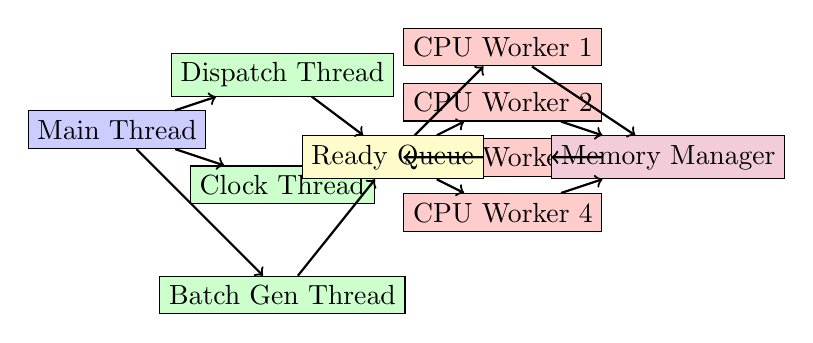
\begin{tikzpicture}[scale=0.7]
            % Main Thread
            \node[draw, rectangle, fill=blue!20] (main) at (0,4) {Main Thread};
            
            % Scheduler Threads
            \node[draw, rectangle, fill=green!20] (dispatch) at (3,5) {Dispatch Thread};
            \node[draw, rectangle, fill=green!20] (clock) at (3,3) {Clock Thread};
            \node[draw, rectangle, fill=green!20] (batch) at (3,1) {Batch Gen Thread};
            
            % CPU Worker Threads
            \node[draw, rectangle, fill=red!20] (cpu1) at (7,5.5) {CPU Worker 1};
            \node[draw, rectangle, fill=red!20] (cpu2) at (7,4.5) {CPU Worker 2};
            \node[draw, rectangle, fill=red!20] (cpu3) at (7,3.5) {CPU Worker 3};
            \node[draw, rectangle, fill=red!20] (cpu4) at (7,2.5) {CPU Worker 4};
            
            % Thread-Safe Queue
            \node[draw, rectangle, fill=yellow!20] (queue) at (5,3.5) {Ready Queue};
            
            % Memory Manager
            \node[draw, rectangle, fill=purple!20] (memory) at (10,3.5) {Memory Manager};
            
            % Arrows
            \draw[->, thick] (main) -- (dispatch);
            \draw[->, thick] (main) -- (clock);
            \draw[->, thick] (main) -- (batch);
            
            \draw[->, thick] (dispatch) -- (queue);
            \draw[->, thick] (batch) -- (queue);
            
            \draw[->, thick] (queue) -- (cpu1);
            \draw[->, thick] (queue) -- (cpu2);
            \draw[->, thick] (queue) -- (cpu3);
            \draw[->, thick] (queue) -- (cpu4);
            
            \draw[->, thick] (cpu1) -- (memory);
            \draw[->, thick] (cpu2) -- (memory);
            \draw[->, thick] (cpu3) -- (memory);
            \draw[->, thick] (cpu4) -- (memory);
        \end{tikzpicture}
    \end{center}
\end{frame}

\begin{frame}[fragile]{Synchronization Mechanisms}
    \textbf{Thread Coordination and Safety}
    \begin{lstlisting}[language=C++]
// Scheduler thread coordination
std::mutex map_mutex_;              // Process map protection
std::mutex finished_mutex_;         // Finished processes
std::mutex memory_mutex_;           // Memory operations
std::condition_variable dispatch_cv_; // Thread notification

// CPU Worker synchronization
std::mutex task_mutex_;             // Task assignment
std::condition_variable task_cv_;   // Worker notification
std::atomic<bool> is_idle_;         // Lock-free state

// Memory Manager synchronization
std::mutex memory_mutex_;           // Virtual memory operations
std::atomic<size_t> pages_paged_in_;  // Statistics counters
std::atomic<size_t> pages_paged_out_; // Lock-free counters
    \end{lstlisting}
    
    \vspace{0.3cm}
    \textbf{Performance Optimizations:}
    \begin{itemize}
        \item Fine-grained locking to minimize contention
        \item Atomic operations for lock-free statistics
        \item Condition variables for efficient thread blocking
    \end{itemize}
\end{frame}

% ======================================================
% SECTION 6: COMMAND INTERFACE
% ======================================================
\section{Command Interface}

\begin{frame}[fragile]{Command System Architecture}
    \textbf{Hash Map-Based Command Processing}
    \begin{lstlisting}[language=C++]
enum class Commands {
    Initialize,      // System configuration loading
    Screen,          // Process management interface
    SchedulerStart,  // Begin batch process generation
    SchedulerStop,   // Stop batch generation
    ReportUtil,      // System utilization report
    Clear,           // Screen clearing
    Exit,            // System shutdown
    ProcessSmi,      // Process memory information
    Vmstat          // Virtual memory statistics
};

// O(1) command lookup via hash map
static const std::unordered_map<std::string, Commands> commands = {
    {"initialize", Commands::Initialize},
    {"scheduler-start", Commands::SchedulerStart},
    {"scheduler-test", Commands::SchedulerStart}, // Alias support
    {"process-smi", Commands::ProcessSmi},
    {"vmstat", Commands::Vmstat}
};
    \end{lstlisting>
\end{frame}

\begin{frame}[fragile]{Screen Command System}
    \textbf{Interactive Process Management}
    \begin{lstlisting}[language=C++]
// Process creation commands
screen -s <name>                    // Create new process
screen -c <name> <size> "<instr>"   // Create with custom instructions
screen -f <name> <file>             // Create from instruction file

// Process monitoring commands
screen -r <name>                    // Resume/view existing process
screen -ls                          // List all processes with status

// Example custom process creation
screen -c myprocess 1024 "DECLARE x 10; ADD y x 5; PRINT(\"Result: \" + y)"
    \end{lstlisting}
    
    \vspace{0.3cm}
    \textbf{Process Status Display:}
    \begin{itemize}
        \item Real-time process log viewing
        \item CPU assignment and execution information
        \item Memory utilization and page fault statistics
        \item Interactive terminal-based interface
    \end{itemize}
\end{frame}

\begin{frame}[fragile]{System Monitoring Commands}
    \textbf{Comprehensive System Statistics}
    \begin{lstlisting}[language=C++]
// Process and Memory Information
process-smi
/*
----------------------------------------------------------------
| PROCESS-SMI V01.00   Driver Version: 01.00                  |
CPU Utilization: 75.23%
Memory Usage: 12288B / 32768B
Memory Util: 37.50%

Running processes and memory usage:
process1    1024B
process2    2048B
----------------------------------------------------------------
*/

// Virtual Memory Statistics  
vmstat
/*
--- vmstat ---
procs -----------memory---------- ---swap-- -----io---- ------cpu-----
 r  b   swpd   free   buff  cache   si   so    bi    bo us sy id wa st
 4  0    512  20480      0      0   15   23     8    12 75 10 15  0  0
-----
Total CPU ticks: 1523
Active ticks: 1145 (75.2%)
Idle ticks: 378 (24.8%)
Memory: 32 K total, 12 K used, 20 K free
Pages: 145 paged in, 89 paged out
*/
    \end{lstlisting>
\end{frame}

% ======================================================
% SECTION 7: CONFIGURATION SYSTEM
% ======================================================
\section{Configuration System}

\begin{frame}[fragile]{Configuration Parameters}
    \textbf{Comprehensive System Configuration}
    \begin{lstlisting}[language=C++]
struct Config {
    uint32_t cpuCount{4};                      // CPU cores (1-128)
    SchedulingAlgorithm scheduler{RoundRobin}; // Scheduling policy
    uint32_t quantumCycles{5};                 // Time quantum
    uint32_t processGenFrequency{1};           // Process creation rate
    uint32_t minInstructions{1000};            // Min process size
    uint32_t maxInstructions{2000};            // Max process size
    uint32_t delayCyclesPerInstruction{0};     // Execution delay
    uint32_t max_overall_mem{16384};           // Total system memory
    uint32_t mem_per_frame{16};                // Frame size
    uint32_t min_mem_per_proc{4096};           // Min process memory
    uint32_t max_mem_per_proc{4096};           // Max process memory
};
    \end{lstlisting}
    
    \vspace{0.3cm}
    \textbf{Validation Features:}
    \begin{itemize}
        \item Power-of-2 validation for memory parameters
        \item CPU count range clamping (1-128 cores)
        \item Dependency validation (quantum cycles for Round Robin)
        \item Default value provision for missing parameters
    \end{itemize}
\end{frame}

\begin{frame}[fragile]{Sample Configuration Files}
    \textbf{Configuration Examples for Different Scenarios}
    
    \textbf{High Performance Configuration:}
    \begin{lstlisting}[basicstyle=\ttfamily\tiny]
num-cpu 8
scheduler "rr"
quantum-cycles 4
batch-process-freq 1
min-ins 1000
max-ins 2000
delay-per-exec 0
max-overall-mem 32768
mem-per-frame 32
min-mem-per-proc 8
max-mem-per-proc 8
    \end{lstlisting}
    
    \textbf{Memory Stress Test Configuration:}
    \begin{lstlisting}[basicstyle=\ttfamily\tiny]
num-cpu 8
scheduler "rr"
quantum-cycles 1
batch-process-freq 1
min-ins 10000
max-ins 10000
delay-per-exec 0
max-overall-mem 1024
mem-per-frame 256
min-mem-per-proc 1024
max-mem-per-proc 1024
    \end{lstlisting}
\end{frame}

% ======================================================
% SECTION 8: ADVANCED FEATURES
% ======================================================
\section{Advanced Features}

\begin{frame}{Virtual Memory System Features}
    \textbf{Advanced Memory Management Capabilities}
    
    \begin{itemize}
        \item \textbf{Demand Paging:} Pages loaded only when accessed
        \begin{itemize}
            \item Lazy loading reduces initial memory overhead
            \item Page fault handling with automatic recovery
            \item Transparent fault resolution during instruction execution
        \end{itemize}
        
        \item \textbf{LRU Page Replacement:} Intelligent eviction algorithm
        \begin{itemize}
            \item Least Recently Used algorithm implementation
            \item Access time tracking for optimal replacement decisions
            \item Minimizes page fault frequency through smart caching
        \end{itemize}
        
        \item \textbf{Backing Store System:} Persistent page storage
        \begin{itemize}
            \item File-based storage for swapped pages
            \item Process isolation through unique offsets
            \item Maintains page contents across swapping operations
        \end{itemize}
        
        \item \textbf{Memory Protection:} Process boundary enforcement
        \begin{itemize}
            \item Virtual address space isolation
            \item Access violation detection and handling
            \item Resource limit enforcement and exception handling
        \end{itemize}
    \end{itemize}
\end{frame}

\begin{frame}{Multi-Core Processing Features}
    \textbf{True Parallel Processing Capabilities}
    
    \begin{itemize}
        \item \textbf{True Parallelism:} Each core runs in separate thread
        \begin{itemize}
            \item Independent CPU worker threads for each core
            \item Concurrent process execution across multiple cores
            \item Real-time performance scaling with core count
        \end{itemize}
        
        \item \textbf{Load Balancing:} Automatic process distribution
        \begin{itemize}
            \item Dynamic core assignment based on availability
            \item Idle core detection and utilization
            \item Optimal resource utilization across all cores
        \end{itemize}
        
        \item \textbf{Core Affinity:} Process-to-core assignment tracking
        \begin{itemize}
            \item Process assignment history maintenance
            \item Core utilization statistics and monitoring
            \item Performance optimization through affinity management
        \end{itemize}
        
        \item \textbf{Scalable Architecture:} Support for up to 128 cores
        \begin{itemize}
            \item Configurable core count with validation
            \item Linear performance scaling with additional cores
            \item Enterprise-level simulation capabilities
        \end{itemize}
    \end{itemize}
\end{frame}

\begin{frame}{Process Scheduling Features}
    \textbf{Advanced Scheduling System Capabilities}
    
    \begin{itemize}
        \item \textbf{Multiple Algorithms:} FCFS and Round-Robin support
        \begin{itemize}
            \item First Come First Served for batch processing
            \item Round-Robin with configurable time quantum
            \item Algorithm selection based on workload characteristics
        \end{itemize}
        
        \item \textbf{Dynamic Generation:} Automatic process creation
        \begin{itemize}
            \item Configurable batch process generation frequency
            \item Random instruction sequence generation
            \item Memory stress testing through hostile programs
        \end{itemize}
        
        \item \textbf{Priority Handling:} Process state management
        \begin{itemize}
            \item Ready, running, and finished state tracking
            \item Process lifecycle management with timestamps
            \item Comprehensive process status reporting
        \end{itemize}
        
        \item \textbf{Statistics Tracking:} Comprehensive utilization monitoring
        \begin{itemize}
            \item CPU utilization calculation and reporting
            \item Process execution time tracking
            \item System performance metrics and analysis
        \end{itemize}
    \end{itemize}
\end{frame}

% ======================================================
% SECTION 9: TESTING AND VALIDATION
% ======================================================
\section{Testing and Validation}

\begin{frame}[fragile]{System Testing Scenarios}
    \textbf{Comprehensive Test Cases}
    
    \textbf{Task 1: Memory Operations Test}
    \begin{lstlisting}[basicstyle=\ttfamily\tiny]
Config: 1 CPU, RR scheduler, quantum 10, 256MB memory
Test: Custom process with DECLARE, ADD, WRITE, READ, PRINT operations
Expected: Correct variable computation and memory operations
    \end{lstlisting}
    
    \textbf{Task 2: High Paging Activity Test}
    \begin{lstlisting}[basicstyle=\ttfamily\tiny]
Config: 8 CPU, 1024MB total, 1024MB per process (only 1 process fits)
Test: scheduler-test for extended period
Expected: High page in/out activity (>min-ins * process_count)
    \end{lstlisting}
    
    \textbf{Task 3: CPU Utilization Variations}
    \begin{lstlisting}[basicstyle=\ttfamily\tiny]
Config: 1 CPU, high batch frequency (60), generous memory (4096MB)
Test: Observe CPU utilization patterns
Expected: Both 100% and 0% CPU utilization scenarios
    \end{lstlisting}
    
    \textbf{Task 4: Process Monitoring}
    \begin{lstlisting}[basicstyle=\ttfamily\tiny]
Config: 4 CPU, 32KB memory, 32-byte frames, 8-byte processes
Test: process-smi, screen -ls, periodic vmstat
Expected: 100% CPU utilization, growing active memory
    \end{lstlisting}
\end{frame}

\begin{frame}[fragile]{Advanced Testing Scenarios}
    \textbf{Stress Testing and Edge Cases}
    
    \textbf{Task 5: Memory Deadlock Scenario}
    \begin{lstlisting}[basicstyle=\ttfamily\tiny]
Config: 8 CPU, 16KB total memory, 32KB per process (impossible fit)
Test: scheduler-test, wait, scheduler-stop, monitor processes
Expected: 0% CPU utilization (deadlock), no process execution
    \end{lstlisting}
    
    \vspace{0.5cm}
    \textbf{Performance Validation Methods:}
    \begin{itemize}
        \item \textbf{Memory Pressure Testing:} Insufficient memory configurations
        \item \textbf{CPU Saturation Testing:} High process generation rates
        \item \textbf{Page Fault Stress Testing:} Hostile program generation
        \item \textbf{Multi-Core Scaling:} Performance measurement across core counts
        \item \textbf{Long-Running Stability:} Extended execution periods
    \end{itemize}
    
    \vspace{0.3cm}
    \textbf{Validation Metrics:}
    \begin{itemize}
        \item CPU utilization accuracy and reporting
        \item Memory allocation and deallocation correctness
        \item Page fault frequency and handling efficiency
        \item Process execution completion rates
        \item System responsiveness under load
    \end{itemize}
\end{frame}

% ======================================================
% SECTION 10: CONCLUSIONS
% ======================================================
\section{Conclusions}

\begin{frame}{System Achievements}
    \textbf{Major Accomplishments}
    
    \begin{itemize}
        \item \textbf{Complete OS Simulation:} Comprehensive operating system emulator
        \begin{itemize}
            \item Virtual memory with demand paging implementation
            \item Multi-core CPU scheduling with load balancing
            \item Process management with comprehensive PCB system
            \item Thread-safe inter-process communication
        \end{itemize}
        
        \item \textbf{Advanced Memory Management:} Enterprise-level features
        \begin{itemize}
            \item LRU page replacement algorithm
            \item File-based backing store system
            \item Process memory isolation and protection
            \item Page fault handling with automatic recovery
        \end{itemize}
        
        \item \textbf{Scalable Architecture:} High-performance design
        \begin{itemize}
            \item Support for up to 128 CPU cores
            \item Thread-safe data structures throughout
            \item Lock-free operations where possible
            \item Fine-grained locking for minimal contention
        \end{itemize}
        
        \item \textbf{Educational Value:} Excellent learning platform
        \begin{itemize}
            \item Real-world OS concepts implementation
            \item Comprehensive documentation and code comments
            \item Configurable parameters for experimentation
            \item Multiple testing scenarios and validation
        \end{itemize}
    \end{itemize}
\end{frame}

\begin{frame}{Technical Excellence}
    \textbf{Design Quality and Implementation}
    
    \begin{itemize}
        \item \textbf{Modern C++ Standards:} C++20 features utilization
        \begin{itemize}
            \item Smart pointers for automatic memory management
            \item Atomic operations for lock-free programming
            \item Template-based generic data structures
            \item Exception handling for robust error recovery
        \end{itemize}
        
        \item \textbf{Software Engineering Best Practices:}
        \begin{itemize}
            \item Modular design with clear separation of concerns
            \item Comprehensive error handling and validation
            \item Extensive documentation and code comments
            \item Consistent coding style and naming conventions
        \end{itemize}
        
        \item \textbf{Performance Optimizations:}
        \begin{itemize}
            \item O(1) command lookup via hash maps
            \item Efficient data structures and algorithms
            \item Memory-efficient page table implementation
            \item Minimal thread contention through fine-grained locking
        \end{itemize}
        
        \item \textbf{Extensibility and Maintainability:}
        \begin{itemize}
            \item Plugin-based architecture for new features
            \item Configuration-driven behavior modification
            \item Clear interfaces between system components
            \item Comprehensive testing framework and scenarios
        \end{itemize}
    \end{itemize}
\end{frame}

\begin{frame}{Future Enhancements}
    \textbf{Potential System Improvements}
    
    \begin{itemize}
        \item \textbf{Enhanced Scheduling Algorithms:}
        \begin{itemize}
            \item Priority-based scheduling implementation
            \item Multi-level feedback queue system
            \item Real-time scheduling with deadline support
            \item Dynamic load balancing algorithms
        \end{itemize}
        
        \item \textbf{Advanced Memory Features:}
        \begin{itemize}
            \item Multiple page replacement algorithms (FIFO, Clock)
            \item Shared memory and inter-process communication
            \item Memory compression and deduplication
            \item NUMA (Non-Uniform Memory Access) simulation
        \end{itemize}
        
        \item \textbf{System Monitoring and Analytics:}
        \begin{itemize}
            \item Real-time performance dashboards
            \item Historical performance data collection
            \item Machine learning-based performance prediction
            \item Automated system tuning and optimization
        \end{itemize}
        
        \item \textbf{Extended Instruction Set:}
        \begin{itemize}
            \item Floating-point arithmetic operations
            \item String manipulation instructions
            \item File I/O operations simulation
            \item Network communication primitives
        \end{itemize}
    \end{itemize}
\end{frame}

\begin{frame}{Final Summary}
    \begin{center}
        \textbf{\Large CSOPESY Operating System Emulator}
        
        \vspace{0.5cm}
        \textbf{\large A Comprehensive OS Simulation Platform}
    \end{center}
    
    \vspace{0.5cm}
    \begin{itemize}
        \item \textbf{Advanced Implementation:} Modern C++20 with enterprise-level features
        \item \textbf{Complete System:} Virtual memory, multi-core scheduling, process management
        \item \textbf{Educational Excellence:} Ideal platform for understanding OS concepts
        \item \textbf{Performance Focus:} Scalable architecture with optimization throughout
        \item \textbf{Extensible Design:} Ready for future enhancements and modifications
    \end{itemize}
    
    \vspace{0.5cm}
    \begin{center}
        \textbf{Developed by the PEGP Team}
        
        Paul Ivan Enclonar, Joel Ethan Batac, Joshua Gilo, Peter Parker
        
        \vspace{0.3cm}
        \textit{Computer Systems Organization and Programming}
    \end{center}
\end{frame}

\begin{frame}
    \begin{center}
        \textbf{\Huge Thank You}
        
        \vspace{1cm}
        \textbf{\Large Questions and Discussion}
        
        \vspace{1cm}
        \textit{CSOPESY Operating System Emulator}
        
        \textit{Advanced OS Concepts Implementation}
    \end{center}
</frame>

\end{document}